\chapter{Auswertung}
\label{chap:Auswertung}
In diesem Kapitel sollen die im Experiment gewonnen Messdaten ausgewertet werden. Bereits bei einer Kalibrationsmessreihe mit Argon konnten aufgrund einer Fehlfunktion der Elektronenkanone keine vollständigen Wirkungsquerschnitte aufgenommen werden. Die Zahl der Elektronen, die für die Berechnung des Wirkungsquerschnittes benötigt werden, kann nicht ausreichend genau eingestellt werden, sodass gerade bei geringeren Energien keine Messung möglich ist. Nach einer Reperatur sollte dies wieder möglich sein. 

Aus diesem Grund kann nur eine qualitative Auswertung einer Kalibrationsmessung mit Argon, sowie eines Restgasspektrums durchgeführt werden. Anschließend folgt eine Simulation der Ionenoptik des Massenspektrometers, mit der alternativ die Genauigkeit des Massenspektrometers überprüft werden kann. Sämtliche Auswertung der Messdaten, sowie alle eigenen Plots in dieser Arbeit wurden mit Python und der \textit{Matplotlib}-Bibliothek erstellt.

\section{Auswertung der Messdaten}
\subsection{Kalibrationsmessung mit Argon}

\subsection{Restgasspektrum}
Eine weitere Möglichkeit zur Überprüfung des Massenspektrometers ist die Aufnahme eines Restgasspektrums. Hierbei wird kein Gas in die Kammer eingelassen und lediglich der atmosphärische Hintergrund in der Kammer gemessen. Dieser besteht aus verschiedenen Restgasen, die durch die Elektronenstoßionisation genauso ionisiert werden können. In einem Vakuum erwartet man vorallem Rückstände von Wassermolekülen, sowie stabiler Kohlenstoffverbindungen, die bei der Vakuumbildung aus den Wänden der Kammer gelöst werden, als auch Reste von Stickstoff und Sauerstoff aus der Luft. Außerdem können besonders leichte Gase, hier vorallem Wasserstoff, übrig bleiben, da sie besonders flüchtig sind und die Vakuumpumpen sie weniger effektiv entfernen können. Es ist zusätzlich praktisch die Restgasverteilung zu kennen, um sie bei der Auswertung von Messungen berücksichtigen zu können. Aufgrund der geringen Dichte und damit niedrigem Ionisierungsquerschnitt muss diese Messung lange durchgeführt werden. 

Wie bereits bei der Kalibrationsmessung muss das Massespektrum neu skaliert werden, um die Masse-zu-Ladungsverhältnisse der Ionen zu bestimmen. Dafür wird für einige der Peaks anhand von den Erwartungen eine Annahme getroffen, welchem Verhältnis sie entsprechen könnten. Für die Identifikation der Ionen wurde angenommen, das der größte Peak ionisierten Wassermolekülen
entspricht und der erste Peak ionisiertem Wasserstoff. Das resultierende, skalierte Restgasspektrum ist in Abb. \ref{fig:rest} dargestellt.

Wie erwartet können die größten Peaks auf ionisierte Wassermoleküle, sowie Wasserstoff zurückgeführt werden. Auch die Peaks von molekularem Stickstoff, Sauerstoff und vermutlich Kohlenstoffdioxid sind gut zu erkennen. Die Struktur und Übereinstimmung des Restgasspektrums zeigen, dass die Anlage korrekt funktioniert und zur Identifikation von Produktionen taugt. Außerdem ist zu erkennen, dass Massendifferenzen von 1 $u$ im Bereich leichter Ionen aufgelöst werden können. 

\begin{figure}
    \centering
    \hspace*{-1cm}
    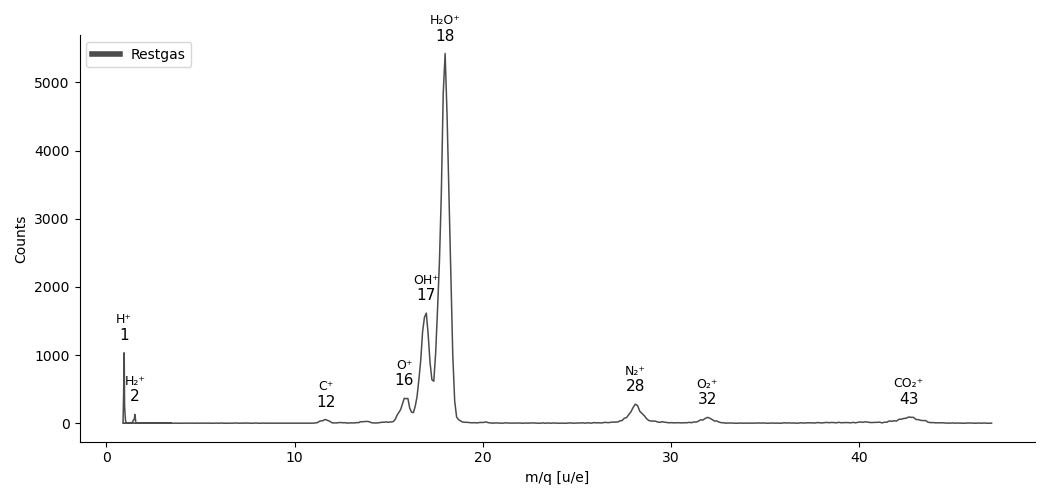
\includegraphics[width=1.05\textwidth]{Restgas.png}
    \caption[Masse-zu-Ladungsspektrum der Restgase]{Masse-zu-Ladungsspektrum der Restgase erzeugt aus dem Flugzeitspektrum in Abb. \ref{fig:rest_tof}. Die Peaks entsprechen den verschiedenen Ionen, die durch die Elektronenstoßionisation entstanden sind. Das Spektrum wurde skaliert, um die Masse zu Ladungsverhältnisse der Ionen zu bestimmen.}
    \label{fig:rest}
\end{figure}

\subsection{Ermittlung des Elektronenstrahlprofils aus den Positionsdaten}
Die Positionen der detektierten Ionen auf dem Detektor können genutzt werden, um das Strahlprofil, also die räumliche Verteilung der Teilchen in einem Schnitt des Strahls, zu bestimmen. Um das Strahlprofil über die ganze abgebildete Länge zu mitteln, wird Daten-Binning genutzt. Das bedeutet, dass für jede y-Koordinate in einem \textit{Bin} die Counts aller detektierten Ionen aufsummiert werden. Das Ergebnis ist ein Histogramm, das die räumliche Verteilung der Elektronen entlange der y-Achse zeigt. Das Ergebnis ist in Abb. \ref{fig:Strahlprofil} dargestellt. Für das Profil des Strahls wird eine Gauß-Verteilung erwartet, da thermische Effekte und Beugung die Position der Elektronen zufällig beeinflussen. Mit einem Fit der Daten mit einer Gauß-Funktion kann die Breite des Strahls bestimmt werden. In der Abbildung ist zu erkennen, dass die Abweichung der Daten vom Fit sehr klein ist. Über die Parameter der gefittetn Funktion kann die volle Breite bei halbem Maximum (FWHM) des Strahls bestimmt werden. Sie beträgt 1.94 mm. 

\begin{figure}
    \centering
    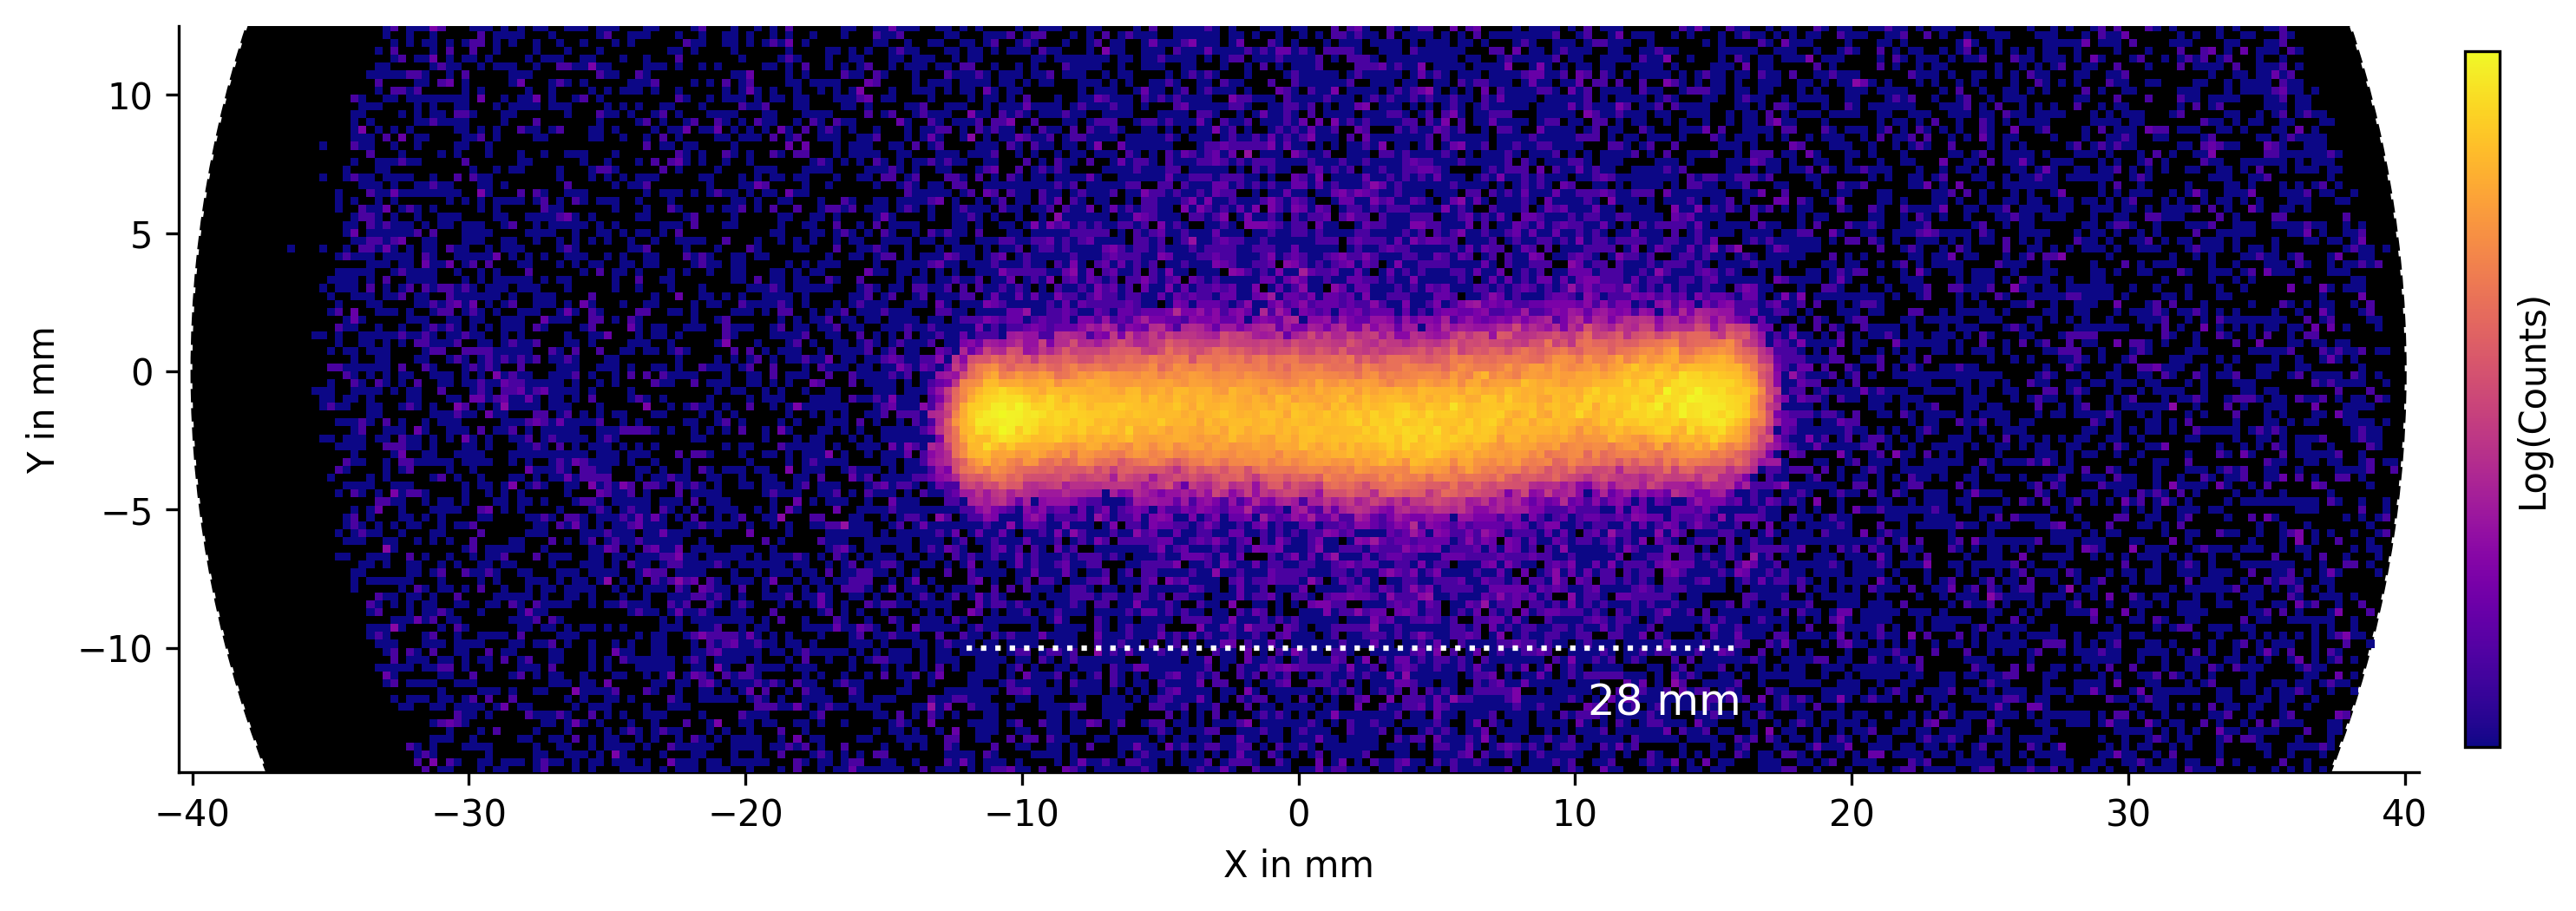
\includegraphics[width=1.05\textwidth]{Strahl.png}
    \caption[Abbild des Strahls auf dem Detektor]{Positionsbestimmung der detektierten Teilche auf dem Detektor zeigen den Strahl auf dem Detektor. Da der Detektor schief verbaut ist, wurde das Bild im Nachhinein gedreht. Das Abbild des Strahls ist seitlich begrenzt, da die Ionen durch das 2 cm große Loch in der Deckenplatte auf den Detektor gelangen.}
    \label{fig:Strahl} 
\end{figure}

\begin{figure}
    \centering
    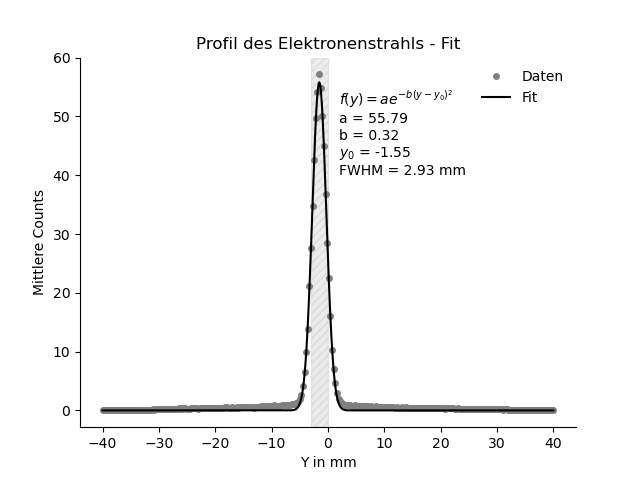
\includegraphics[width=1\textwidth]{Strahlprofil.png}
    \caption[Gemitteltes Strahlprofil]{Gemitteltes Strahlprofil aus den Positionen der detektierten Ionen. Die Daten wurden mit einem Gaußfit gefittet, um die Breite des Strahls zu bestimmen. In grau-schraffiert eingezeichnet ist die volle Breite bei halbem Maximum (FWHM) des Strahls abgebildet.}
    \label{fig:Strahlprofil} 
\end{figure}